\chapter{Presentazione del caso di studio}\label{chp:presentazione}
Il sistema oggetto dell'analisi in questione eroga le seguenti tipologie di servizi:
\begin{enumerate}
\item \uo{} (e.g. ricarica \textsl{PostePay}, invio raccomandata e pagamento di massimo tre bollettini)
\item \pp{} (e.g. pagamento di un numero arbitrario di bollettini, bollo auto e libretti)  
\item \sr{} (e.g. invio corrispondenza, lettere, pacchi e raccomandate)
\end{enumerate}

Per essere serviti i clienti possono recarsi all'ufficio postale, prendere un ticket relativo al servizio a cui sono interessati e mettersi in coda in attesa del proprio turno. Nel caso in cui essi dimostrino di essere titolari di un conto \textsl{BancoPosta} potranno accodarsi in una fila dedicata.

Un insieme di sportelli serve le richieste degli utenti in accordo alle seguenti regole: 
\begin{enumerate}[label=R\arabic*), align=left, leftmargin=*]
\item I ticket di tipo \sr{} vengono serviti da uno sportello dedicato il quale, in assenza di questa tipologia, opera come gli altri. Il comportamento di tale servente è schematizzato in figura \ref{fig:presentazione-1}. 
\item Poiché, per definizione, ticket di tipo \uo{} dovrebbero richiedere meno tempo per essere processati, viene assegnata loro una priorità maggiore di \pp{}.
\item I clienti titolari di un conto \textsl{BancoPosta} vengono serviti con una priorità maggiore rispetto agli altri, in accordo alle regole R1 ed R2.
\end{enumerate}

\begin{figure}[ht]
\centering
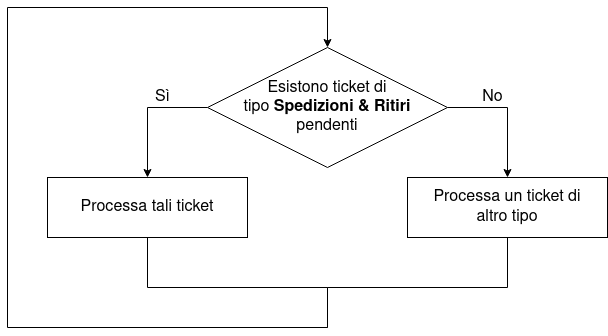
\includegraphics[width=0.75\linewidth]{presentazione-1}
\caption{Schema del comportamento del servente dedicato ai ticket di tipo \sr}
\label{fig:presentazione-1}
\end{figure}

Il periodo di erogazione dei ticket è pari a 8 ore, al termine delle quali vengono processate ugualmente le richieste rimaste pendenti. Questo implica che nel momento in cui un cliente entra in possesso di un ticket, la sua richiesta verrà sicuramente servita prima della chisura. 

In definitiva, la giornata lavorativa dell'ufficio postale è costituita dall'unione del periodo d'erogazione e dal tempo necessario allo smaltimento delle richieste in coda.
